\documentclass[10pt, a4paper, twocolumn]{article}
\usepackage{graphicx}
\usepackage{float}
\usepackage{amsmath}

\title{Reconciling organizational cost across business units}
\author{Mya Pitzeruse}

\begin{document}
\maketitle

\begin{abstract}
  This paper describes a solution to reconcile cost for shared infrastructure across business units.
  It was designed to be comprehensive and flexible.
  The original target for the solution was a hybrid-cloud infrastructure.
  As a result, it's concepts are generic and support both cloud and non-cloud ecosystems.
  The goal of the solution is to attribute costs appropriately across a spectrum of platforms.
\end{abstract}


\section*{Introduction}
  Products run across a variety of platforms.
  Many use a combination of platforms to perform work efficiently.
  Figure~\ref{figure:1} demonstrates how you might use platforms like Apache Hadoop, Kubernetes, and other managed services to build a product.

  \begin{figure}[H]
    \centering
    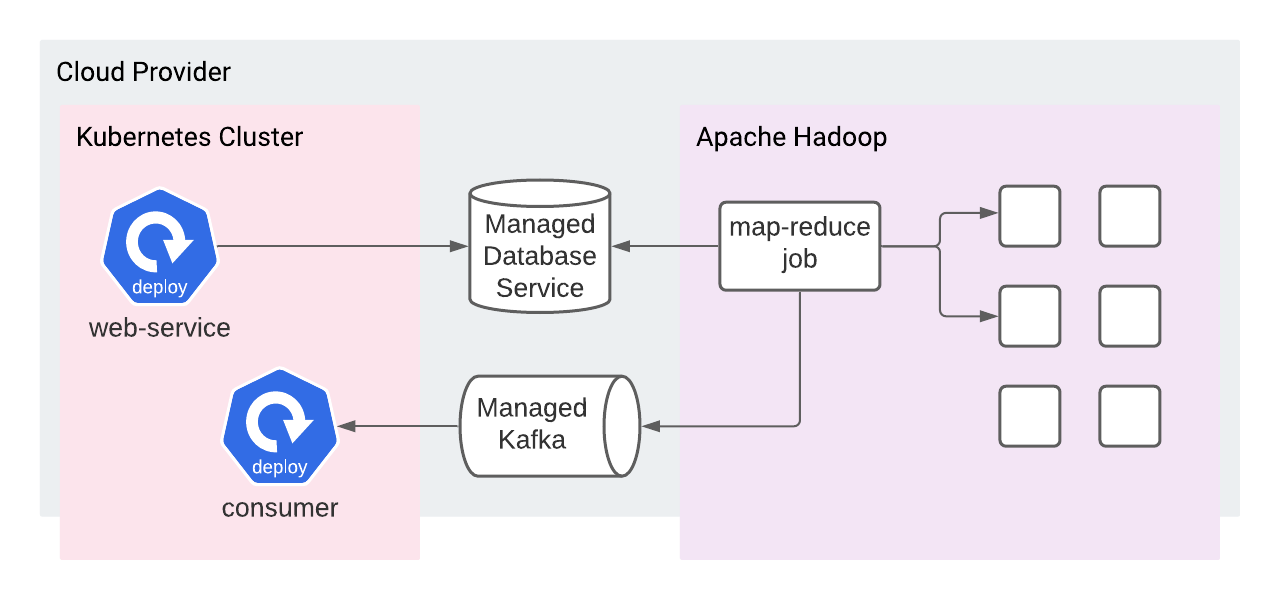
\includegraphics[width=\linewidth]{./truth-and-reconciliation-application.png}
    \caption{A multiple platform application}
    \label{figure:1}
  \end{figure}

  When an organization is small, they're often less concerned about attributing spend to their products.
  As an organization grows, they often add new products to complement their existing offerings.
  With each new product, this figure grows more complex.
  As this figure grows more complex, the need to attributing spend increases as well.
  Executives often want to know how much each of their products cost to run and what their return on investment is.
  When asked for this information, engineering leaders need to take time to track down all this information.

  Solutions like \textit{CloudTamer} help organizations better manage their spend on cloud providers, but lack visibility into clustered environments.
  In cluster solutions like \textit{kubecost} provide visibility into the cost of Kubernetes pods, but miss managed services.
  In the end, you wind up back to where you started.
  Needing to query multiple sources for information.

  While these account for common cases, it fails to consider less common ones.
  Suppose one part of your organization runs a service on behalf of the rest.
  You might want to apportion usage of that service out to it's heaviest consumers.
  Throughout the course of my research, I found that no (if not few) comprehensive solutions exist.
  In designing a comprehensive solution, I wanted to ensure compatibility with many existing solutions.


\section*{Background}
  In November 2018, I re-joined Indeed to help with their ongoing Kubernetes effort.
  At the time, we were feeling some pain-points scaling our Apache Mesos based infrastructure.
  Some efforts towards a Kubernetes based ecosystem had been underway.

  The first effort was geared toward a short-term migration.
  It would allow us to move off Apache Mesos while preserving the overall structure of our ecosystem.
  The second was tasked with figuring out how to run upstream Kubernetes safely and securely.
  As we migrated to Kubernetes, teams built out some cost attribution.
  The hope was to report on changes in products between platforms as well as provide transparency to resource use.

  Similar questions were raised as we began our journey to the the cloud.
  During this time, I considered several solutions.
  Many of them were geared toward solving in cluster or out of cluster costs, not both.
  In working with the CNCF end user group, I learned many organizations share similar positions.
  Either they were looking for a more comprehensive solution or were using multiple to fill in the gaps.
  At the time, my focus at work was pretty deep into this space.

  In discovering a lack of comprehensive solutions, I researched as much as I could.
  I looked to open source to see what solutions did well and what they were missing.
  I looked at the data we were already reporting and how I could build off that.
  In doing soIn doing so, I was able to identify commonalities across each of them.

  \begin{itemize}
    \item Products are composed of one or more workloads
    \item Workloads have an identifier (often unique to the platform) and require resources to run
    \item Resources between each data set varied with some commonality (CPU, memory, disk)
    \item Each data set represented an exchange of services between one group and their customers
  \end{itemize}

  These discoveries lead to the design a development of a common reporting platform.
  The platform is designed with decomposition in mind.
  It allows additional layers to be added progressively, allowing organizations to add granularity over time.

\section*{Concepts}
  This section contains concepts that are fundamental to the solution.
  Understanding them will help map them to potential internal concepts.

  \subsection*{Workloads}
    Products are composed of one or more workloads.
    Workloads represent a variety of processes an organization might run.
    They can be a long running, public facing web services or background jobs.
    Workloads can run across a variety of platforms but are often deployed to just one.

  \subsection*{Resources}
    Workloads require resources to run.
    Common cases need things like CPU, memory, and occasionally disk.
    At the same time, it's important that resources are made available through a variety of platforms.
    Kubernetes allows containers to reserve resources and it finds room within the cluster to run.
    Similarly, virtual machines can be used to allocate resources, while also providing virtualized hardware.
    Regardless of where and how the workloads run, resources are uniform.
    They are measured using standardized units and typically come at some cost.

  \subsection*{Standard Units of Measure}
    With anything we measure, standardization and documentation of units is important.
    Without it, one group might code against one standard while another codes using a second.
    Some standardized units of measure include:

    \begin{itemize}
      \item \textbf{CPU} is measured in \textbf{millicores}
      \item \textbf{GPU} is measured in \textbf{cores}
      \item \textbf{Memory} is measured in \textbf{bytes}
      \item \textbf{Disk} is measured in \textbf{bytes} and \textbf{iops}
      \item \textbf{Transport} is measured in \textbf{bytes}
      \item \textbf{Time} is measured in \textbf{milliseconds}
      \item An \textbf{API} is measured in \textbf{requests per second}
    \end{itemize}

    Finer grained units can be used if needed.

  \subsection*{Uniform Resource Names}
    A uniform resource name (URN) is like a uniform resource identifier (URI).
    They were developed early on in the days of the internet.
    URNs should be:

    \begin{itemize}
      \item Globally unique
      \item Persistent
      \item Location-independent
      \item Namespaced
    \end{itemize}

    To help understand this concept a bit more, let's consider an example using RFCs.
    The following URN is for RFC-2141, the specification for URNs.

\begin{verbatim}
  urn:ietf:rfc:2141
\end{verbatim}

    This URN uses the \textit{ietf} namespace with the \textit{rfc} namespace-specific string.
    In order to ensure global uniqueness, namespaces must be registered with the Internet Assigned Numbers Authority (IANA.)
    Since most organizations will keep this information internally, the need to register the namespace is less of a requirement.
    For simplicity, we will use the \textit{costrecon} namespace.
    This namespace has \textbf{not} been registered and only serves as demonstration.

    A URN in this document refers to specific workloads.
    Let us consider a database deployment MySQL name appdb.
    At some point, I might want to migrate appdb from MySQL to PostgreSQL.
    During this time, both a MySQL and PostgreSQL resource will exist with the name appdb.
    As a result, you should scope your identifiers appropriately.
    The block below enumerates several examples of further namespacing by class and kind.

\begin{verbatim}
  urn:costrecon:aws:642135246531
  urn:costrecon:compute:host:appname
  urn:costrecon:compute:vm:appname
  urn:costrecon:compute:pod:appname
  urn:costrecon:compute:container:appname
  urn:costrecon:storage:postgres:appdb
  urn:costrecon:storage:mysql:appdb
  urn:costrecon:storage:rds:appdb
  urn:costrecon:storage:aurora:appdb
  urn:costrecon:storage:spanner:appdb
\end{verbatim}

    \subsubsection*{Amazon's ARN}
      Amazon leverages it's own resource naming scheme called ARNs.
      Similar to URNs, ARNs represent a unique resource in AWS.
      The solution described herein should support ARNs in place of URNs.
      It's recommended that URNs are consistent in implementations for simplicity and ease of use.

  \subsection*{Double-entry Bookkeeping}
    Double-entry bookkeeping is a common practice used by most (if not all) financially regulated systems.
    It is used to keep accounts balanced and as an error detection tool.
    Implementation of such a system requires several key details:

    \begin{itemize}
      \item Each entry added is immutable.
      \item Every entry added to one account, requires a corresponding entry in the other account.
      \item Both charges (debits) and payments (credits) are tracked independently.
    \end{itemize}

    Double-entry systems are often implemented as a ledger.
    This allows the system to track transactions for a given account.
    In this solution, we augment the traditional approach to double-entry bookkeeping with hierarchy.
    This is done to model the real-world exchange of resources between groups.
    Consider Figure~\ref{figure:2}.

    \begin{figure}[H]
      \centering
      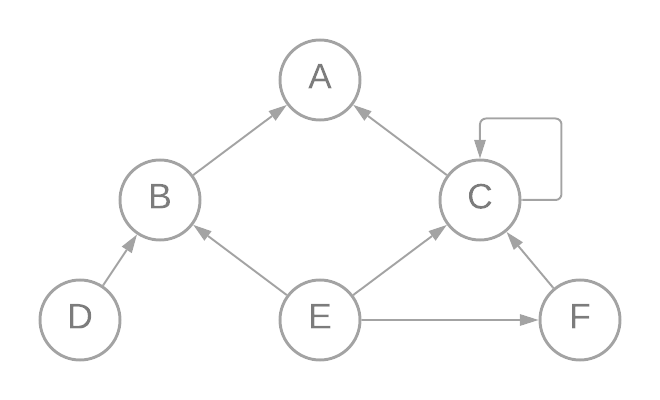
\includegraphics[width=\linewidth]{./truth-and-reconciliation-graph.png}
      \caption{Exchange of service graph}
      \label{figure:2}
    \end{figure}

    This graph shows how projects can build upon one another to deliver value to the business.
    For example, E uses services provided by B, C, and F.
    At the end of the day, we want to ensure E is attributed the resources that they consume.

\section*{Implementation}
  When it comes to implementation, I've found there are two schools fo thought.

  The first approach is to use real world dollars.
  This encounters many challenges such as choosing a base currency or determining the cost of non-cloud environments.
  In many ways, this information is extremely valuable for product owners.
  They understand what their system costs and how much they should expect to charge for their service.
  In the wrong hands, this information is dangerous.

  The second approach is to use a basis point type of system.
  This approach allows you to represent the underlying usage as a percentage.
  One problem with this approach is that when you scale a cluster up, usage goes down.
  This is because the increase in available resources changes what percentage of the cluster you use.
  This can be really confusing if you haven't deployed changes recently.

  At the end of the day, we need a combination of approaches.
  Basis points should be used to apportion out usage at each tier.
  When displaying or analyzing information, a currency value should be used.
  This approach allows for the most accurate representation of a given products cost.

  \subsection*{Apportioning Usage}
    Apportioning usage of a platform is the process of dividing a single pool of resources amongst consumers.
    This is done using basis points in order to address issues with things like over-commit.
    When using a non-basis point model, over-commit often results in an over-charge of resources.
    This means that a given product could become cashflow-positive.
    While this may be the goal of any user facing product, it's often not the goal of apportioning.

    In order to establish the proper basis points, we must first know what the total available resources are.
    This is done by taking the maximum of what is available (common case) and what is reserved (over-commit).
    This will need to be done across all resources you want to apportion out.
    The equations below can be used to compute the total availability of a given resource.

    \begin{gather*}
      T_{reserved} = \sum^{workloads}_{W} max(W_{reserved}, W_{usage}) \\
      \\
      T = max(T_{available}, T_{reserved}) \\
    \end{gather*}

    Once you've computed the total amount of a given resource, you should be able to start distributing basis points.
    The equation below demonstrates how to calculate basis points for a single resource for a single workload.

    \begin{gather*}
      basispoints = \frac{max(reserved, usage)}{T} * 100 \\
    \end{gather*}

    At the end, we have a set of basis points for each resource we want to charge for.
    We need to convert this set of basis points to a single basis point.
    Since we know the sample size for each resource group is the same, we can safely use an average.
    Let us consider the following allocations.

    \begin{itemize}
      \item \textbf{10000} basis points from GPU reservations
      \item \textbf{1000} basis points from CPU reservations
      \item \textbf{3000} basis points from memory reservations
    \end{itemize}

    The above workload averages out with \textbf{4667} basis points.
    Suppose this workload ran in a shared cluster with one other workload.
    That workload claims the remaining resources (0 GPU, 9000 CPU, 7000 memory) which averages \textbf{5333} basis points.
    Together, they sum to \textbf{10000} or 100\%.
    This will allow us to annotate every edge with a single weight.

    \begin{figure}[H]
      \centering
      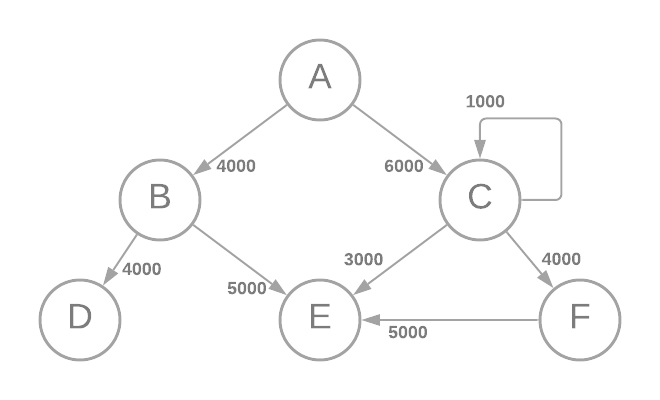
\includegraphics[width=\linewidth]{./truth-and-reconciliation-graph-weighted.png}
      \caption{Weighted exchange of service graph}
      \label{figure:3}
    \end{figure}

  \subsection*{Apportioning Cost}
    As said earlier, apportioning usage is not enough.
    There needs to be able to be a monetary value.
    Now, this monetary value could be a real value, like a bill.
    Or, it could be a synthetic value that someone made up.

    It works by attaching a cost to a root workload in the graph.
    From there, all subsequent charges can be derived using common, well known algorithms.

    \subsubsection*{Path Enumeration}
      In many cases, we want to know the cost of a single product.
      Path enumeration is used to provide a list of all paths between a pair of vertices in a graph.
      This same concept can be applied using a single starting vertex and a direction to search.
      The following is a path enumeration for \textit{A} in Figure~\ref{figure:3}.

      \begin{enumerate}
        \item A, B, D
        \item A, B, E
        \item A, C, E
        \item A, C, F, E
      \end{enumerate}

      Similarly, this can be applied in the opposite direction.
      The following is an inverse path enumeration for \textit{E}.

      \begin{enumerate}
        \item E, B, A
        \item E, C, A
        \item E, F, C, A
      \end{enumerate}

      Path enumeration is key to attributing cost.

    \subsubsection*{Computing Cost}
      Using the enumerated paths, we can compute the total cost for a given workload.
      Costs are computed using the weights on the edge of the graph in combination with root costs.
      The equations are as follows.

      \begin{gather*}
        \forall^{workloads}_{w} \\
        \\
        cost(w) = \sum^{paths}_{p} cost(p) \\
        \\
        cost(p) = root(p) \times \prod^{p}_{edge} (weight / 10000) \\
        \\
        root(p) = p[len(p) - 1]_{cost} \\
      \end{gather*}

      To help explain, let's consider \textit{D}.
      It has a single path, \textit{D, B, A}.
      Figure~\ref{figure:4} highlights this path in blue.

      \begin{figure}[H]
        \centering
        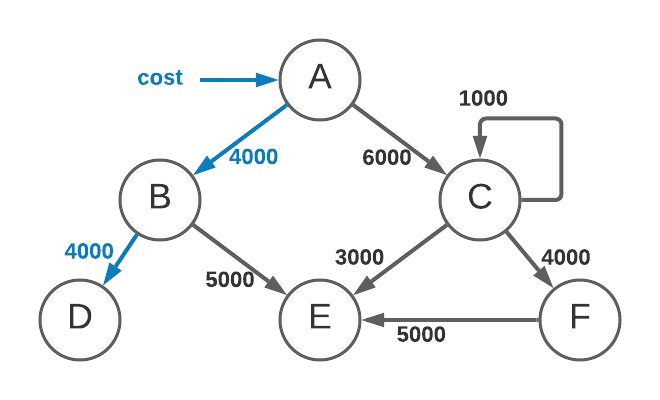
\includegraphics[width=\linewidth]{./truth-and-reconciliation-cost-d.png}
        \caption{p1 for D}
        \label{figure:4}
      \end{figure}

      Using the information in the graph and our equations, we can compute a cost for \textit{D}.

      \begin{gather*}
        cost(p_{1}) = A_{cost} \times 0.4 \times 0.4 \\
        \\
        cost(D) = A_{cost} \times 0.16 \\
      \end{gather*}

      If \textit{A} costs \textbf{100 USD}, then \textit{D} costs \textbf{16 USD}.
      Similarly, we can consider a more complicated example.
      \textit{E} has three paths.
      They are documented in the section on Path Enumeration and
      highlighted in Figures~\ref{figure:5},~\ref{figure:6},~and~\ref{figure:7}.

      \begin{figure}[H]
        \centering
        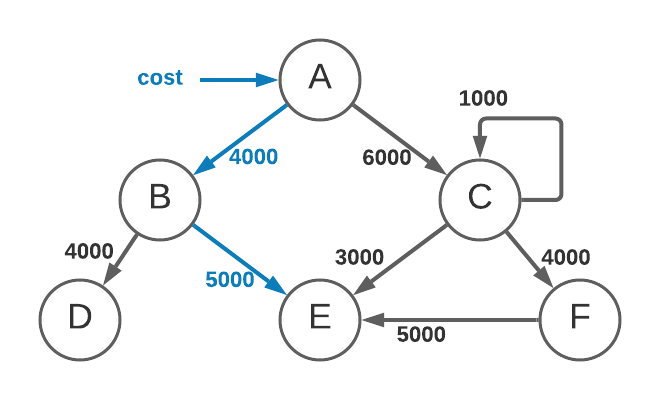
\includegraphics[width=\linewidth]{./truth-and-reconciliation-cost-ep1.png}
        \caption{p1 for E}
        \label{figure:5}
      \end{figure}

      \begin{figure}[H]
        \centering
        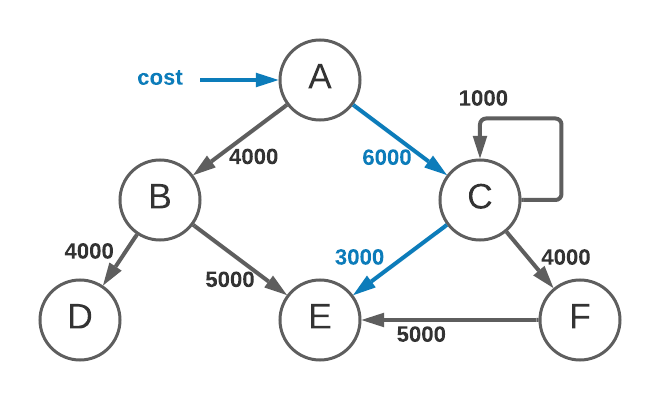
\includegraphics[width=\linewidth]{./truth-and-reconciliation-cost-ep2.png}
        \caption{p2 for E}
        \label{figure:6}
      \end{figure}

      \begin{figure}[H]
        \centering
        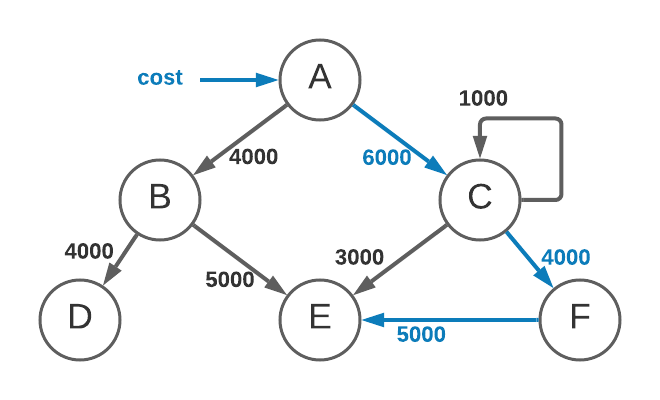
\includegraphics[width=\linewidth]{./truth-and-reconciliation-cost-ep3.png}
        \caption{p3 for E}
        \label{figure:7}
      \end{figure}

      While more complicated, the process is the same.

      \begin{gather*}
        cost(p_{1}) = A_{cost} \times 0.4 \times 0.5 \\
        cost(p_{2}) = A_{cost} \times 0.6 \times 0.3 \\
        cost(p_{3}) = A_{cost} \times 0.6 \times 0.4 \times 0.5 \\
        \\
        cost(E) = A_{cost} \times (0.2 + 0.18 + 0.12) \\
        cost(E) = A_{cost} \times 0.5 \\
      \end{gather*}

      If \textit{A} costs \textbf{100 USD}, then \textit{E} costs \textbf{50 USD}.

  \subsection*{Reconciling Cost}
    As we are dealing with a system that apportions cost, we should ensure that the apportioning is done correctly.
    In accounting, reconciliation is used to ensure that the money leaving an account matches the actual money spent.
    We can use the same process to balance our computed costs against the provided costs.
    Table~\ref{table:1} demonstrates how the accounts are balanced using their attributed cost and billable claims.

    \begin{table}[H]
      \centering
      \begin{tabular}{ l|c|r|c }
        $w$ & Attributed       & Billable & Balance \\
        \hline
        A   & $ x            $ &    10000 & $ 0 $ \\
        B   & $ x \times .4  $ &     9000 & $ x \times 0.04 $ \\
        C   & $ x \times .6  $ &     7000 & $ x \times 0.18 $ \\
        D   & $ x \times .16 $ &        0 & $ x \times 0.16 $ \\
        E   & $ x \times .5  $ &        0 & $ x \times 0.50 $ \\
        F   & $ x \times .24 $ &     5000 & $ x \times 0.12 $ \\
        \hline
            &                  &          & $ x \times 1.00 $ \\
      \end{tabular}
      \caption{Reconciliation}
      \label{table:1}
    \end{table}

    This is done using the following equation.

    \[ balance(w) = attributed \times \left(1 - \frac{billable}{10000}\right) \]

    At the end, you have a balance for each project.
    They should sum to the total cost fed into the system (as shown in Table~\ref{table:1}.)
    Since cost is distributed proportionately, we're able to ensure attribution throughout the system.

  \subsection*{The Ledger}

    \begin{table}[H]
      \centering
      \begin{tabular}{ l|l }
        Field & Explanation \\
        \hline
        datetime & Time of transaction \\
        region & A geographic identifier \\
        env & An environmental identifier \\
        payer & Who received services (from) \\
        payee & Who provides services (to) \\
        type & A debit or credit \\
        usage & The usage \\
        urn & A uniform resource name \\
        tags & Organization specific metadata \\
        detail & A break down of charges \\
      \end{tabular}
      \caption{Fields}
      \label{table:2}
    \end{table}

    \begin{table}[H]
      \centering
      \begin{tabular}{ l|l }
        Field & Type \\
        \hline
        datetime & datetime, int64 \\
        region & string \\
        env & string \\
        payer & string \\
        payee & string \\
        type & enum(debit, credit) \\
        usage & int16 \\
        urn & string \\
        tags & map[string]string \\
        detail & map[string]string \\
      \end{tabular}
      \caption{Field types}
      \label{table:3}
    \end{table}

\section*{Closing Remarks}

\end{document}
